\chapter{Experiments}
\label{ch:intro}

In order to evaluate our extension of ILP, the correlation and lattice, and the different interestingness measures, we
perform a series of experiments on Linked Data.

In the first experiment, we compare different measures by building same-sized correlation lattices on the
$hasIncome(X,Y)$ relation from the USCensus, then searching for interesting rules with intervals for $Y$ inside the
lattice itself as described in Section~\ref{sec:searchRulesInCL}. The lattices are build by greedily choosing the top-k
most interesting nodes in each level according to the chosen measure, and pruning the rest so that all the lattices have
the same quantity of nodes.

Also, we measure the total time spent for the construction of each lattice, as well as the number of interesting rules
found on them. As candidate categorical relations, we chose the 18 shown in Table~\ref{tab:uscensusRelations}. More
details about the categories can be found at the PUMS
Data
Dictionary\footnote{\url{http://www.census.gov/acs/www/Downloads/data_documentation/pums/DataDict/PUMSDataDict05_07.pdf}
}

\begin{table}[h!]
\begin{minipage}{\textwidth}
 \begin{center}
 \caption{Chosen categorical relations from USCensus}
  \begin{tabular}{l l c}
    \toprule
      Name	& Label				& Number of Categories \\
    \midrule
      sex	& Sex				&	2	\\
      st	& State				&	52\footnote{Including Puerto Rico and Washington D.C.}	\\
      racwht	& is White			&	2	\\
      racblk	& is Black			&	2	\\
      racasn	& is Asian			&	2	\\
      qtrbir	& Quarter of Birth		&	4	\\	
      nativity	& born In the US		&	2	\\
      mar	& Marital Status		&	5	\\
      lanp	& Language Spoken at Home	&	104	\\
      esr	& Employment Status		&	6	\\
      dphy	& Physical Difficulty		&	2	\\
      schl	& Educational Level		&	17	\\	
      occp	& Occupation			&	470	\\
      sch	& School Enrollment		&	3	\\
      rel	& Relationship (to household owner)		&	12	\\
      esp	& Employment Status of Parents	&	8	\\
      oc	& Own Child			&	2	\\
    \bottomrule
  \end{tabular}
 \label{tab:uscensusRelations}
 \end{center}
\end{minipage}
\end{table}

We build the lattice on a training partition of USCensus of size 1.7GB containing $884365$ people entities, and test the
learned rules on a test set of size 0.4GB with $369024$ people entities. Therewith, we can evaluate the accuracy of the
learned rules. 

The plot from Figure~\ref{fig:uscensus:Nodes-GoodRules} shows the number of rules learned per lattice size (defined by
number of nodes per level). The KL-divergence only has the worst performance, as expected, since clauses with lower
support are more likely to have higher interestingness. The other three measures perform roughly similarly, however, for
fewer nodes, it performs worse than others catching up later. This can be explained by the fact that it gives
preference to very high support categories which cover the majority of the population, such as $hasDeficiency(X,no)$,
which tend to have a distribution similar to its superpopulation. 

Analysing the plot from Figure~\ref{fig:uscensus:Nodes-Runtime}, it is clear that using support only as interestingness
measure has a high cost. As it concentrates on larger categories, the queries required for building the lattice are much
more expensive. JS-divergence and L-divergenc combined with support are much more efficient than support only, as they
can learn about the same amount of rules with on average less than  


Since the USCensus data is completely joined on person entities, and all categorical relations have literals
as constants (usually integer numbers mapped to a set of entities), therefore allowing only star-join patterns, we
chose DBpedia and LinkedMDB in order to evaluate our ILP-extension.

\begin{figure}
\caption{Comparison of number of interesting rules learned per lattice size}
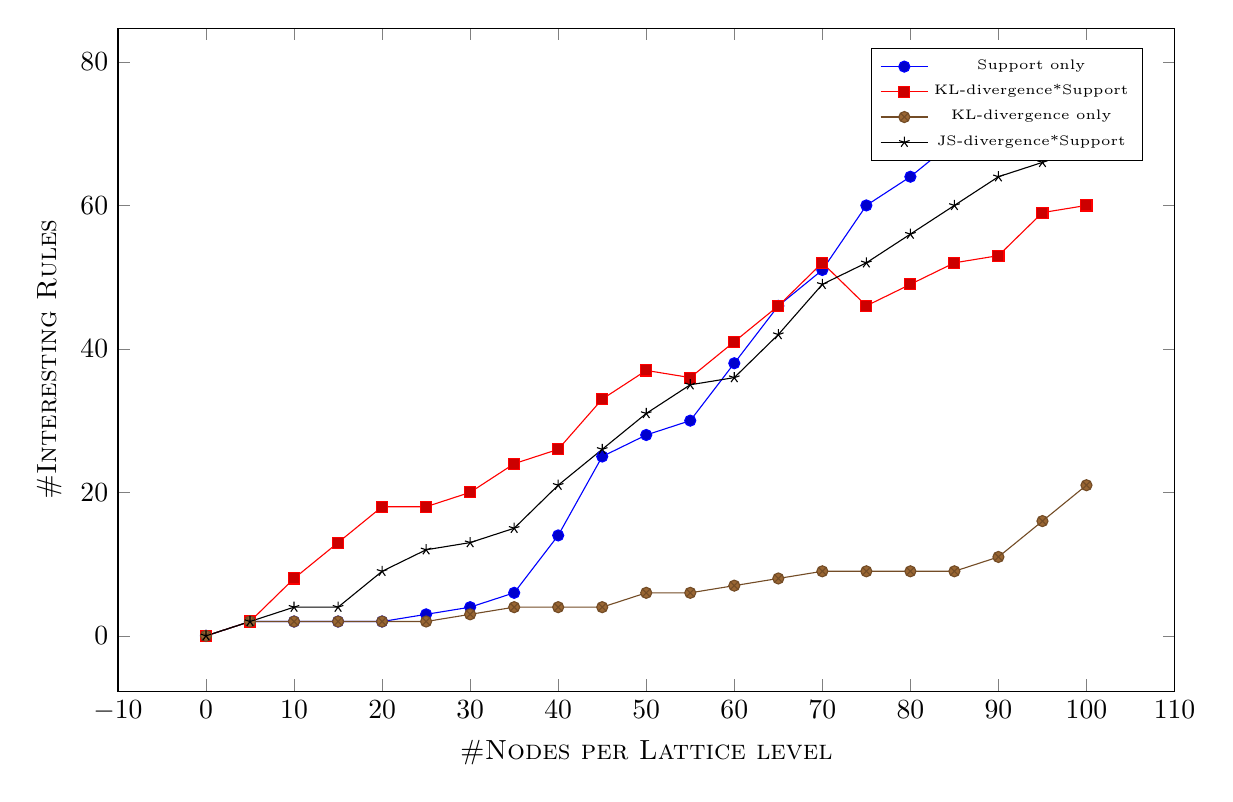
\begin{tikzpicture}[scale=1.0]
 \begin{axis}[
	width=15cm, height=10cm,
        xlabel=\textsc{\#Nodes per Lattice level},
        ylabel=\textsc{\#Interesting Rules},
        legend entries={Support only, KL-divergence*Support, KL-divergence only, JS-divergence*Support},
	legend style={legend pos=north east,font=\tiny}]
    ]
% Support
\addplot coordinates {(0,0) (5,2) (10,2) (15,2) (20,2) (25,3) (30,4) (35,6) (40,14) (45,25) (50,28) (55,30) (60,38)
(65,46) (70,51) (75,60) (80,64) (85,69) (90,71) (95,75) (100,77)};
% KLDiv*Support
\addplot coordinates {(0,0) (5,2) (10,8) (15,13) (20,18) (25,18) (30,20) (35,24) (40,26) (45,33) (50,37) (55,36) (60,41)
(65,46) (70,52) (75,46) (80,49) (85,52) (90,53) (95,59) (100,60)};
% KLDiv Only
\addplot coordinates {(0,0)  (5,2) (10,2) (15,2) (20,2) (25,2) (30,3) (35,4) (40,4) (45,4) (50,6) (55,6) (60,7) (65,8)
(70,9) (75,9) (80,9) (85,9) (90,11) (95,16) (100,21)};
% JS*Support
\addplot coordinates {(0,0)  (5,2) (10,4) (15,4) (20,9) (25,12) (30,13) (35,15) (40,21) (45,26) (50,31) (55,35) (60,36)
(65,42) (70,49) (75,52) (80,56) (85,60) (90,64) (95,66) (100,69)};
\end{axis}
\end{tikzpicture}
\label{fig:uscensus:Nodes-GoodRules}
\end{figure}

\begin{figure}
\caption{Comparison of Correlation Lattice build time per lattice size}
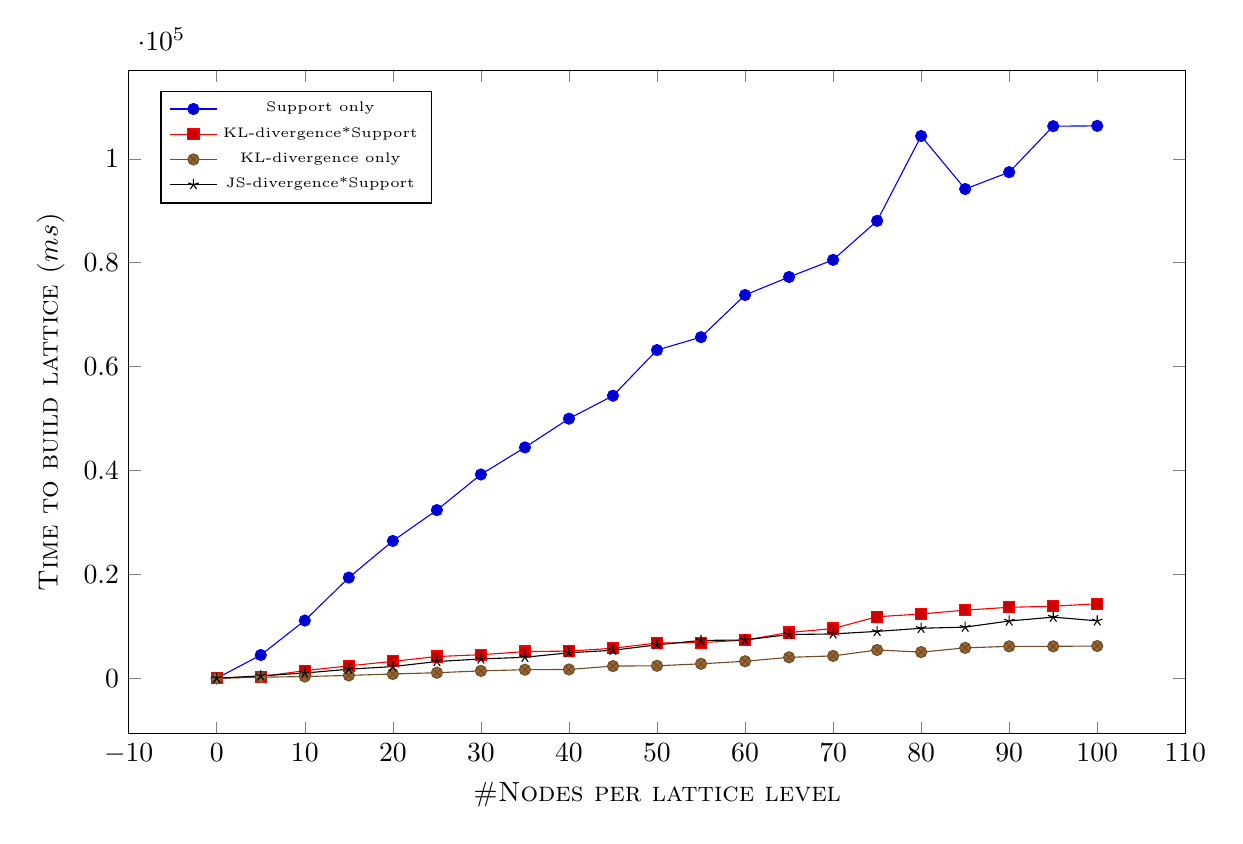
\begin{tikzpicture}[scale=1.0]
 \begin{axis}[
	width=15cm, height=10cm,
        xlabel=\textsc{\#Nodes per lattice level},
        ylabel=\textsc{Time to build lattice ($ms$)},
        legend entries={Support only, KL-divergence*Support, KL-divergence only, JS-divergence*Support},
	legend style={legend pos=north west,font=\tiny}]
    ]
\addplot coordinates {(0,0) (5,4471) (10,11113) (15,19383) (20,26432) (25,32374) (30,39228) (35,44439) (40,49974)
(45,54391) (50,63178) (55,65673) (60,73782) (65,77245) (70,80542) (75,88055) (80,104386) (85,94183) (90,97424)
(95,106279) (100,106336)};
\addplot coordinates {(0,0)  (5,321) (10,1463) (15,2390) (20,3253) (25,4184) (30,4529) (35,5137) (40,5231) (45,5774)
(50,6786) (55,6864) (60,7347) (65,8813) (70,9567) (75,11844) (80,12372) (85,13119) (90,13659) (95,13859) (100,14353)};
\addplot coordinates {(0,0)  (5,207) (10,329) (15,549) (20,825) (25,1065) (30,1420) (35,1652
) (40,1695) (45,2343) (50,2402) (55,2782) (60,3273) (65,4031) (70,4299) (75,5448) (80,5035) (85,5847) (90,6145)
(95,6146) (100,6208)};
\addplot coordinates {(0,0)  (5,466) (10,1011) (15,1746) (20,2253) (25,3220) (30,3717) (35,4042) (40,4904) (45,5390)
(50,6436) (55,7280) (60,7371) (65,8412) (70,8535) (75,9025) (80,9624) (85,9845) (90,11027) (95,11772) (100,11050)};
\end{axis}
\end{tikzpicture}
\label{fig:uscensus:Nodes-Runtime}
\end{figure}

\begin{figure}
\caption{Comparison of number of interesting rules per runtime per lattice size}
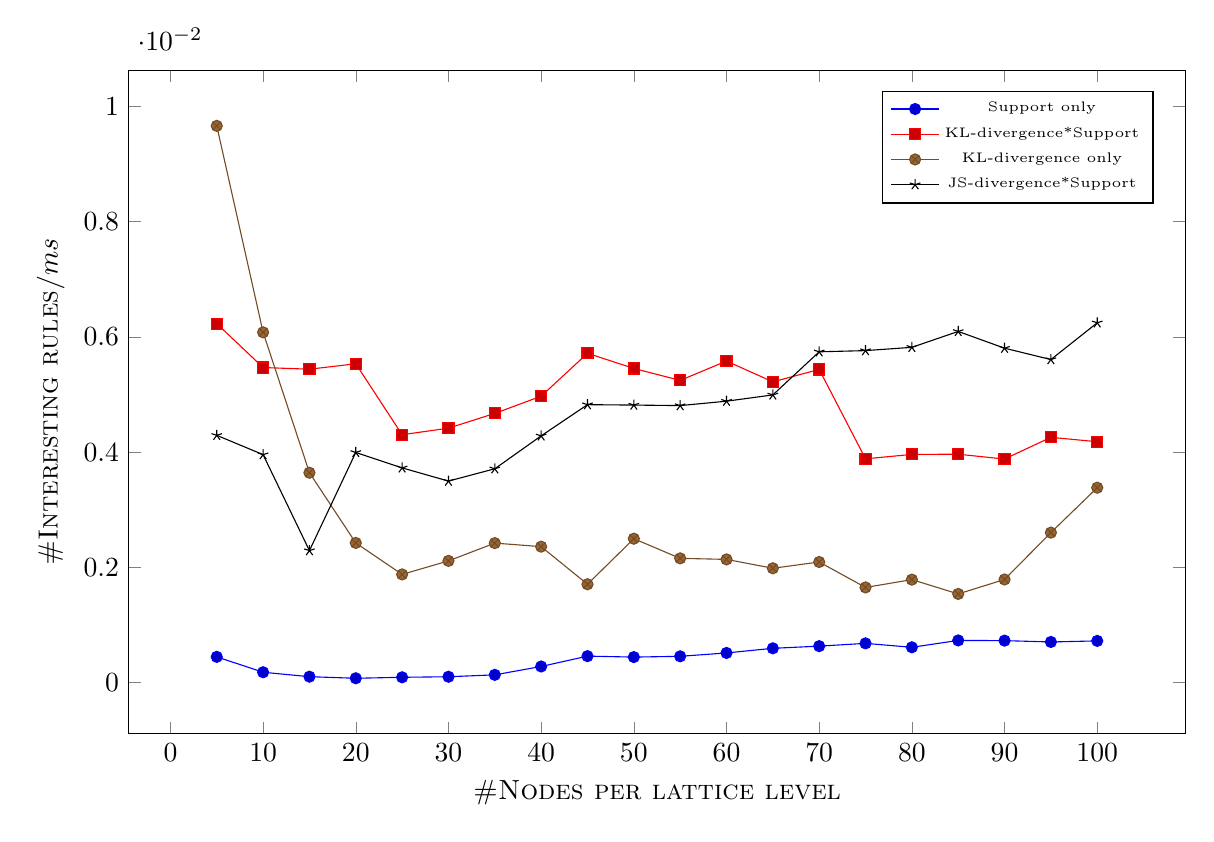
\begin{tikzpicture}[scale=1.0]
 \begin{axis}[
	width=15cm, height=10cm,
        xlabel=\textsc{\#Nodes per lattice level},
        ylabel=\textsc{\#Interesting rules/$ms$},
        legend entries={Support only, KL-divergence*Support, KL-divergence only, JS-divergence*Support},
	legend style={legend pos=north east,font=\tiny}]
    ]
\addplot coordinates {(5,0.0004473272) (10,0.0001799694) (15,0.0001031832) (20,7.566586e-05) (25 ,
9.266695e-05) (30,0.0001019680) (35,0.0001350165) (40,0.0002801457) (45,0.0004596349) (50 ,
0.0004431923) (55,0.0004568087) (60,0.0005150308) (65,0.0005955078) (70,0.00063321) (75,0.0006813923
) (80,0.000613109) (85,0.0007326163) (90,0.0007287732) (95,0.0007056897) (100,0.0007241198)};
\addplot coordinates {(5,0.00623053) (10,0.005468216) (15,0.005439331) (20,0.005533354) (25 ,
0.004302103) (30,0.004415986) (35,0.004671988) (40,0.004970369) (45,0.005715275) (50,0.005452402) (
55,0.005244755) (60,0.005580509) (65,0.005219562) (70,0.005435351) (75,0.003883823) (80 ,
0.003960556) (85,0.003963717) (90,0.003880225) (95,0.004257161) (100,0.004180311)};
\addplot coordinates {(5,0.009661836) (10,0.006079027) (15,0.003642987) (20,0.002424242) (25 ,
0.001877934) (30,0.002112676) (35,0.002421308) (40,0.002359882) (45,0.001707213) (50,0.002497918) (
55,0.002156722) (60,0.002138711) (65,0.001984619) (70,0.00209351) (75,0.001651982) (80,0.001787488
) (85,0.001539251) (90,0.001790073) (95,0.002603319) (100,0.003382732)};
\addplot coordinates {(5,0.004291845) (10,0.003956479) (15,0.002290951) (20,0.003994674) (25 ,
0.003726708) (30,0.003497444) (35,0.003711034) (40,0.004282219) (45,0.004823748) (50,0.004816656) (
55,0.004807692) (60,0.004884005) (65,0.004992867) (70,0.005741066) (75,0.005761773) (80 ,
0.005818786) (85,0.006094464) (90,0.005803936) (95,0.005606524) (100,0.006244344)};
\end{axis}
\end{tikzpicture}
\label{fig:uscensus:Nodes-RulesPerRuntime}
\end{figure}





In our second experiment, we test our proposed approach on LinkedMDB and DBpedia. We merge both datasets onto a single
RDF3X database, create correlation lattices for the properties $budget$ and $runtime$ with categorical relations:
$director$, $writer$, $producer$, $distributor$, $starring$, $country$, and $subject$. We build a pair lattices for each
of the 4 interestingness measures we evaluate: Kullback-Leibler divergence only, Kullback-Leibler combined with support,
Jensen-Shannon combined with support, and support only

Subsequently, we run the ILP with our proposed extension and learn rules with the relation $country$ as head. We
measure the number of base-rules evaluated as interesting, the runtime spent with their search, and how many of the
rules evaluated as interesting actually had an interesting refined-rule. It is important to point out that the
core-ILP runtime, excluding the search for rules with numerical intervals, is the same for all of them measures and
threshold values. 

This is done for the 4 aforementioned measures and various different threshold values. With that we can obtain evaluate
the accuracy and recall of our interestingness predictions, as well as evaluate their efficiency by comparing the amount
of rules learned per runtime.

In this experiment, we used equal frequencies as discretization technique, since the numerical properties are skewed and
quite noisy, with the property $budget$, for instance, containing significant outliers with order of magnitude up to
$10^{14}$.

In this experiment, we do not partition the data into training and test sets in order to evaluate the learned rules,
since the data has a much more complex structure, making the partitioning much trickier than on USCensus, and unfeasible
due to the limited time available. Instead, we simply check the precision of our interestingness predictions, by
counting the number of chosen rules which 

The results obtained in this experiment are not very significant, as the size of $budget$ relation is
not very large (9565 facts). Because of that, it is very difficult to learn a significant amount of rules with fairly
high confidence and support values, therefore many of the learned rules are result of noise.

Figure~\ref{fig:mdbpedia:budget:Precision-Recall} shows how a comparative precision-recall graph for the same 4
interestingness measures. Again, the support only have a relatively good overall performance, however its precision is
bad for low recall values, with all the other measures having better results. In graph from
Figure~\ref{fig:mdbpedia:budget:Precision-Recall}, we notice that the number of rules learned per runtime is better
than linear growth for all the measures with JS-divergence and KL-divergence combined with support outperforming the
other measures, indicating their effectiveness as pruning heuristics.

For the $runtime$ property, on the other hand, we can observe in the graph from
Figure~\ref{fig:mdbpedia:runtime:Runtime-LearnedRules} that this growth is much less steep, being much closer to
linearity for all the measures. To some extent, this difference can be explained by the weaker correlation between the
$runtime$ property and the candidate relations when compared to $budget$. 


\begin{figure}
 \caption{Precision-Recall graph of our interestingness prediction for learning the relation $country$ with
numerical interval for the property $budget$ on LinkedMDB and DBpedia}
 \centering
 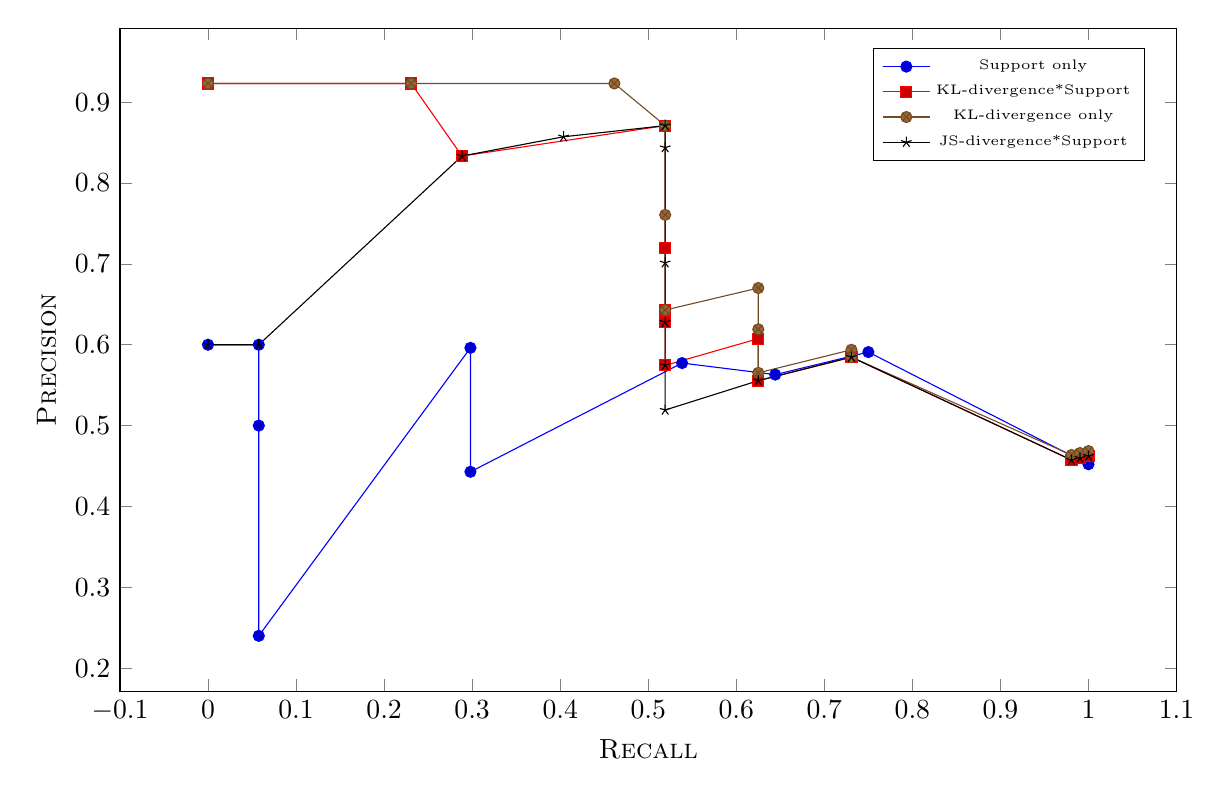
\begin{tikzpicture}[scale=1.0]
  \begin{axis}[
	width=15cm, height=10cm,
	xlabel=\textsc{Recall},
	ylabel=\textsc{Precision},
        legend entries={Support only, KL-divergence*Support, KL-divergence only, JS-divergence*Support},
	legend style={legend pos=north east,font=\tiny}]
      ]
  \addplot coordinates {(0.0,0.6) (0.05769231,0.6) (0.05769231,0.5) (0.05769231,0.24) (0.2980769 ,
0.5961539) (0.2980769,0.4428571) (0.5384616,0.5773196) (0.6442308,0.5630252) (0.75,0.5909091) (1 ,
0.4521739)};

  \addplot coordinates { (0.0,0.9230769) (0.2307692,0.9230769) (0.2884615,0.8333333) (0.5192308,0.8709678)
(0.5192308,0.72) (0.5192308,0.6428571) (0.5192308,0.627907) (0.5192308,0.5744681) (0.625,0.6074766)
(0.625,0.5555556) (0.7307692,0.5846154) (0.9807692,0.4573991) (0.9903846,0.4598214) (1.0,0.4622222)};

\addplot coordinates {(0.0,0.9230769) (0.2307692,0.9230769) (0.4615385,0.9230769) (0.5192308,0.8709678)
(0.5192308,0.7605634) (0.5192308,0.6428571) (0.625,0.6701031) (0.625,0.6190476) (0.625,0.5652174) (
0.7307692,0.59375) (0.7307692,0.5846154) (0.9807692,0.4636364) (0.9903846,0.4660633) (1.0,0.4684685)};

  \addplot coordinates {(0.0,0.6) (0.05769231,0.6) (0.2884615,0.8333333) (0.4038461,0.8571429) (0.5192308
, 0.8709678) (0.5192308,0.84375) (0.5192308,0.7012987) (0.5192308,0.627907) (0.5192308,0.5744681) (
0.5192308,0.5192308) (0.625,0.5555556) (0.7307692,0.5846154) (0.9807692,0.4573991) (0.9903846 ,
0.4598214) (1.0,0.4622222)};
  \end{axis}
  \end{tikzpicture}
\label{fig:mdbpedia:budget:Precision-Recall}
\end{figure}


\begin{figure}
%\begin{minipage}{1\linewidth}\centering
 \caption{Runtime-LearnedRules}
 \centering
 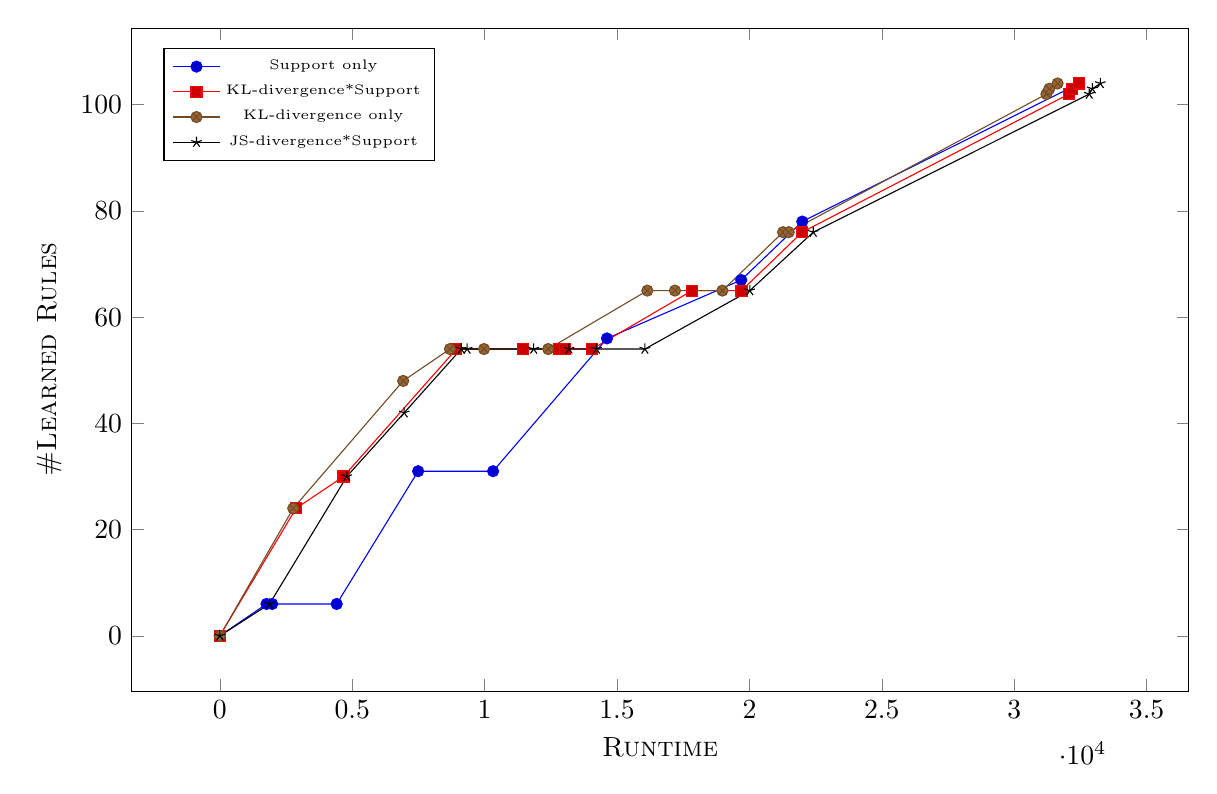
\begin{tikzpicture}
  \begin{axis}[
	width=15cm, height=10cm,
	xlabel=\textsc{Runtime},
	ylabel=\textsc{\#Learned Rules},
        legend entries={Support only, KL-divergence*Support, KL-divergence only, JS-divergence*Support},
	legend style={legend pos=north west,font=\tiny}]
      ]
  \addplot coordinates { (0.0,0.0) (1762,6) (1976,6) (4413,6) (7488,31) (10319,31) (14620,56) (
19691,67) (21995,78) (32452,104)};

  \addplot coordinates {(0.0,0.0) (2877,24) (4672,30) (8934,54) (11447,54) (12813,54) (13033,54)
(14057,54) (17836,65) (19703,65) (21991,76) (32064,102) (32173,103) (32449,104)};

  \addplot coordinates {(0.0,0.0) (2772,24) (6923,48) (8690,54) (9977,54) (12400,54) (16145,65)
(17187,65) (18979,65) (21270,76) (21483,76) (31215,102) (31324,103) (31637,104)};

  \addplot coordinates {(0.0,0.0) (1877,6) (4795,30) (6962,42) (9116,54) (9337,54) (11852,54) (
13187,54) (14225,54) (16052,54) (20014,65) (22411,76) (32833,102) (32949,103) (33251,104
)};
  \end{axis}
  \end{tikzpicture}
 % \end{minipage}
\label{fig:mdbpedia:budget:Runtime-LearnedRules}
\end{figure}




\begin{figure}
 \caption{Precision-Recall comparison of our interestingness prediction for learning the relation $country$ with
numerical interval for the property $runtime$ on LinkedMDB and DBpedia}
 \centering
 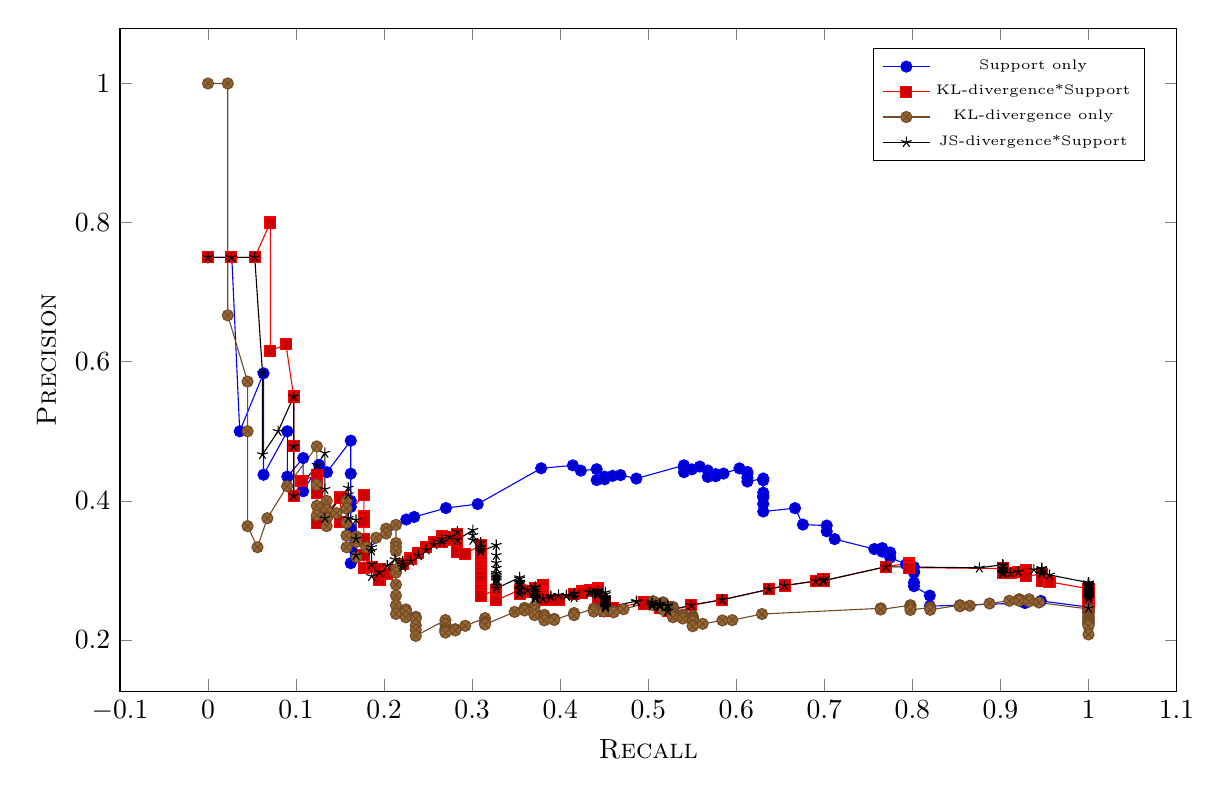
\begin{tikzpicture}[scale=1.0]
  \begin{axis}[
	width=15cm, height=10cm,
	xlabel=\textsc{Recall},
	ylabel=\textsc{Precision},
        legend entries={Support only, KL-divergence*Support, KL-divergence only, JS-divergence*Support},
	legend style={legend pos=north east,font=\tiny}]
      ]
  \addplot coordinates {(0,0.75) (0.02702703,0.75) (0.03603604,0.5) (0.06306306,0.5833333) (0.06306306,0.4375)
(0.09009009,0.5) (0.09009009,0.4347826) (0.1081081,0.4615385) (0.1081081,0.4137931) (0.1261261,0.4516129)
(0.1351351,0.4411765) (0.1621622,0.4864865) (0.1621622,0.4390244) (0.1621622,0.4) (0.1621622,0.3913043) (0.1621622,0.36)
(0.1621622,0.3333333) (0.1621622,0.3103448) (0.1711712,0.3220339) (0.2252252,0.3731343) (0.2342342,0.3768116)
(0.2702703,0.3896104) (0.3063063,0.3953488) (0.3783784,0.4468085) (0.4144144,0.4509804) (0.4234234,0.4433962)
(0.4414415,0.4454545) (0.4414415,0.4298246) (0.4504505,0.4347826) (0.4504505,0.4310345) (0.4594594,0.4358974)
(0.4684685,0.4369748) (0.4864865,0.432) (0.5405405,0.4511278) (0.5405405,0.4477612) (0.5405405,0.4411765)
(0.5495495,0.4452555) (0.5585586,0.4492754) (0.5675676,0.443662) (0.5675676,0.4344827) (0.5765766,0.4383562)
(0.5765766,0.4353741) (0.5855856,0.4391892) (0.6036036,0.4466667) (0.6126126,0.4415584) (0.6126126,0.4387097)
(0.6126126,0.433121) (0.6126126,0.4276729) (0.6306306,0.4320988) (0.6306306,0.4294479) (0.6306306,0.4117647)
(0.6306306,0.4069767) (0.6306306,0.4046243) (0.6306306,0.3954802) (0.6306306,0.3846154) (0.6666667,0.3894737)
(0.6756757,0.3658537) (0.7027027,0.364486) (0.7027027,0.3561644) (0.7117117,0.3449781) (0.7567568,0.3307086)
(0.7657658,0.3320312) (0.7657658,0.3269231) (0.7747748,0.3257576) (0.7747748,0.3245283) (0.7747748,0.3185185)
(0.7927928,0.3087719) (0.8018018,0.3047945) (0.8018018,0.2986577) (0.8018018,0.2966666) (0.8018018,0.2825397)
(0.8018018,0.2772586) (0.8198198,0.2637681) (0.8198198,0.2486339) (0.9279279,0.2530713) (0.9459459,0.2560976)
(1,0.2472160)};

  \addplot coordinates {(0,0.75) (0.02654867,0.75) (0.05309734,0.75) (0.07079646,0.8) (0.07079646,0.6153846)
(0.08849558,0.625) (0.09734514,0.55) (0.09734514,0.4782609) (0.09734514,0.4074074) (0.1061947,0.4285714)
(0.1238938,0.4375) (0.1238938,0.4242424) (0.1238938,0.4117647) (0.1238938,0.3684211) (0.1504425,0.4047619)
(0.1504425,0.3695652) (0.1769912,0.4081633) (0.1769912,0.3773585) (0.1769912,0.3703704) (0.1769912,0.3448276)
(0.1769912,0.3225806) (0.1769912,0.3030303) (0.1858407,0.3043478) (0.1946903,0.3013699) (0.1946903,0.2857143)
(0.2035398,0.2948718) (0.2123894,0.3) (0.2212389,0.308642) (0.2300885,0.3170732) (0.2389381,0.3253012)
(0.2477876,0.3333333) (0.2566372,0.3411765) (0.2654867,0.3488372) (0.2654867,0.3409091) (0.2743363,0.3483146)
(0.2743363,0.3444445) (0.2831858,0.3516484) (0.2831858,0.3478261) (0.2831858,0.3368421) (0.2831858,0.3333333)
(0.2831858,0.3265306) (0.2920354,0.3235294) (0.3097345,0.3365385) (0.3097345,0.3333333) (0.3097345,0.3181818)
(0.3097345,0.3153153) (0.3097345,0.3125) (0.3097345,0.3070175) (0.3097345,0.3017241) (0.3097345,0.2991453)
(0.3097345,0.2966102) (0.3097345,0.2916667) (0.3097345,0.2845528) (0.3097345,0.2755905) (0.3097345,0.2734375)
(0.3097345,0.2713178) (0.3097345,0.2671756) (0.3097345,0.2651515) (0.3097345,0.2631579) (0.3274336,0.2720588)
(0.3274336,0.270073) (0.3274336,0.2642857) (0.3274336,0.2624114) (0.3274336,0.2569444) (0.3539823,0.2721089)
(0.3539823,0.2666667) (0.3628319,0.2697369) (0.3716814,0.2745098) (0.380531,0.2792208) (0.380531,0.275641)
(0.380531,0.2704402) (0.380531,0.26875) (0.380531,0.2670807) (0.380531,0.2654321) (0.380531,0.2638037)
(0.380531,0.2606060) (0.380531,0.2590362) (0.380531,0.2574850) (0.3893805,0.2573099) (0.3982301,0.2571429)
(0.4159292,0.2655367) (0.4247788,0.2696629) (0.4247788,0.2681564) (0.4336283,0.2722222) (0.4336283,0.2707182)
(0.4424779,0.2747253) (0.4424779,0.2732241) (0.4424779,0.2717391) (0.4424779,0.2673797) (0.4424779,0.2631579)
(0.4424779,0.2617801) (0.4424779,0.2604167) (0.4424779,0.2590674) (0.4424779,0.2577319) (0.4424779,0.2564103)
(0.4424779,0.2551020) (0.4424779,0.2525252) (0.4424779,0.25) (0.4513274,0.2537313) (0.4513274,0.2524753)
(0.4513274,0.2512315) (0.4513274,0.25) (0.4513274,0.2487805) (0.4513274,0.2475728) (0.4513274,0.2463768)
(0.4513274,0.2451923) (0.4513274,0.2428571) (0.4513274,0.2417062) (0.460177,0.245283) (0.4955752,0.2545455)
(0.4955752,0.2522523) (0.5132743,0.2521739) (0.5132743,0.2510822) (0.5132743,0.25) (0.5132743,0.2489270)
(0.5132743,0.2468085) (0.5132743,0.2457627) (0.5221239,0.2478992) (0.5221239,0.2418033) (0.5486726,0.25)
(0.5840708,0.2578125) (0.6371682,0.2727273) (0.6548672,0.2781955) (0.6902655,0.2846715) (0.699115,0.2872727)
(0.699115,0.2851986) (0.7699115,0.3052632) (0.7964602,0.3103448) (0.7964602,0.3092783) (0.7964602,0.3082192)
(0.7964602,0.3040541) (0.9026549,0.3026706) (0.9026549,0.3008850) (0.9026549,0.2982456) (0.9026549,0.2965116)
(0.9115045,0.2968300) (0.9115045,0.2959770) (0.920354,0.2979943) (0.9292035,0.3) (0.9292035,0.2991453)
(0.9292035,0.2957746) (0.9292035,0.2924791) (0.9292035,0.2916667) (0.9469026,0.2947658) (0.9469026,0.2931507)
(0.9469026,0.2915531) (0.9469026,0.2907609) (0.9469026,0.2899729) (0.9469026,0.2891892) (0.9469026,0.2853333)
(0.9557522,0.2834646) (1,0.2736078) (1,0.2729469) (1,0.2722892) (1,0.2703349) (1,0.2696897) (1,0.2677725) (1,0.2671395)
(1,0.2665094) (1,0.264637) (1,0.2634033) (1,0.262181) (1,0.2603687) (1,0.2591743) (1,0.2456522)};

  \addplot coordinates {(0,1) (0.02247191,1) (0.02247191,0.6666667) (0.04494382,0.5714286) (0.04494382,0.5)
(0.04494382,0.3636364) (0.05617978,0.3333333) (0.06741573,0.375) (0.08988764,0.4210526) (0.1235955,0.4782609)
(0.1235955,0.4230769) (0.1235955,0.3928571) (0.1235955,0.3793103) (0.1348315,0.4) (0.1348315,0.3870968)
(0.1348315,0.375) (0.1348315,0.3636364) (0.1460674,0.3823530) (0.1573034,0.4) (0.1573034,0.3888889)
(0.1573034,0.3684211) (0.1573034,0.35) (0.1573034,0.3333333) (0.1685393,0.3488372) (0.1685393,0.3409091)
(0.1685393,0.3191489) (0.1797753,0.3333333) (0.1910112,0.3469388) (0.2022472,0.36) (0.2022472,0.3529412)
(0.2134831,0.3653846) (0.2134831,0.3392857) (0.2134831,0.3333333) (0.2134831,0.3275862) (0.2134831,0.3015873)
(0.2134831,0.296875) (0.2134831,0.2794118) (0.2134831,0.2638889) (0.2134831,0.25) (0.2134831,0.2375)
(0.2247191,0.2439024) (0.2247191,0.2409639) (0.2247191,0.2325581) (0.2359551,0.2333333) (0.2359551,0.2307692)
(0.2359551,0.2210526) (0.2359551,0.2142857) (0.2359551,0.2058824) (0.2696629,0.2285714) (0.2696629,0.2222222)
(0.2696629,0.2162162) (0.2696629,0.2142857) (0.2696629,0.2123894) (0.2696629,0.2105263) (0.2808989,0.2155172)
(0.2808989,0.2136752) (0.2921348,0.220339) (0.3146068,0.2314050) (0.3146068,0.2258064) (0.3146068,0.224)
(0.3146068,0.2222222) (0.3483146,0.2403101) (0.3595506,0.2461539) (0.3595506,0.2442748) (0.3595506,0.2424243)
(0.3707865,0.2481203) (0.3707865,0.2426471) (0.3707865,0.2357143) (0.3820225,0.2361111) (0.3820225,0.2328767)
(0.3820225,0.2281879) (0.3932584,0.2302632) (0.3932584,0.2287582) (0.4157303,0.2387097) (0.4157303,0.2356688)
(0.4382023,0.245283) (0.4382023,0.24375) (0.4382023,0.2407408) (0.4494382,0.2409639) (0.4606742,0.2411765)
(0.4606742,0.2397661) (0.4719101,0.2441860) (0.505618,0.2556818) (0.505618,0.2513967) (0.505618,0.25)
(0.5168539,0.2541437) (0.5168539,0.2527473) (0.5168539,0.2513661) (0.5168539,0.2486486) (0.5168539,0.2473118)
(0.5168539,0.2446809) (0.5168539,0.2433862) (0.5280899,0.2473684) (0.5280899,0.2460733) (0.5280899,0.2447917)
(0.5280899,0.2435233) (0.5280899,0.2397959) (0.5280899,0.2385787) (0.5280899,0.2373737) (0.5280899,0.2361809)
(0.5280899,0.235) (0.5280899,0.2338308) (0.5280899,0.2326733) (0.5393258,0.2364532) (0.5393258,0.2341463)
(0.5393258,0.2318841) (0.5393258,0.2307692) (0.5505618,0.2344498) (0.5505618,0.2322275) (0.5505618,0.2311321)
(0.5505618,0.2300469) (0.5505618,0.2289720) (0.5505618,0.2268518) (0.5505618,0.2207207) (0.5505618,0.2197309)
(0.5617977,0.2232143) (0.5842696,0.2280702) (0.5955056,0.2284483) (0.6292135,0.2372881) (0.764045,0.2454874)
(0.764045,0.2437276) (0.7977528,0.25) (0.7977528,0.2491228) (0.7977528,0.2465278) (0.7977528,0.2431507)
(0.8202247,0.2466216) (0.8202247,0.2457912) (0.8202247,0.2433333) (0.8539326,0.25) (0.8539326,0.248366)
(0.8651685,0.2491909) (0.8876405,0.2523962) (0.9101124,0.2563291) (0.9213483,0.2586751) (0.9213483,0.2570533)
(0.9213483,0.25625) (0.9325843,0.258567) (0.9325843,0.2553846) (0.9438202,0.2537764) (1,0.2445055) (1,0.2438356)
(1,0.2425068) (1,0.2398922) (1,0.2392473) (1,0.2379679) (1,0.2348285) (1,0.2342105) (1,0.2335958) (1,0.2317708)
(1,0.2311688) (1,0.2305699) (1,0.2299742) (1,0.2282051) (1,0.2276215) (1,0.2258883) (1,0.2253165) (1,0.2241814)
(1,0.2230576) (1,0.2213930) (1,0.220297) (1,0.2079439) };

  \addplot coordinates {(0,0.75) (0.02654867,0.75) (0.05309734,0.75) (0.0619469,0.5833333) (0.0619469,0.4666667)
(0.07964602,0.5) (0.09734514,0.55) (0.09734514,0.4782609) (0.09734514,0.4074074) (0.1238938,0.4516129)
(0.1327434,0.46875) (0.1327434,0.4166667) (0.1327434,0.375) (0.1592920,0.4186046) (0.1592920,0.4090909)
(0.1592920,0.375) (0.1681416,0.372549) (0.1681416,0.3454545) (0.1681416,0.3220339) (0.1858407,0.3333333)
(0.1858407,0.328125) (0.1858407,0.3088235) (0.1858407,0.2916667) (0.1946903,0.2972973) (0.2035398,0.3066667)
(0.2123894,0.3157895) (0.2212389,0.3125) (0.2212389,0.308642) (0.2212389,0.3048781) (0.2300885,0.313253)
(0.2389381,0.3214286) (0.2477876,0.3294118) (0.2566372,0.3372093) (0.2654867,0.3448276) (0.2654867,0.3409091)
(0.2743363,0.3483146) (0.2831858,0.3555556) (0.2831858,0.344086) (0.3008850,0.3578947) (0.3008850,0.3505155)
(0.3008850,0.3434343) (0.3097345,0.3398058) (0.3097345,0.3333333) (0.3097345,0.3301887) (0.3097345,0.3271028)
(0.3274336,0.3363636) (0.3274336,0.3217391) (0.3274336,0.3109244) (0.3274336,0.3032787) (0.3274336,0.296)
(0.3274336,0.2936508) (0.3274336,0.2913386) (0.3274336,0.2890625) (0.3274336,0.2868217) (0.3274336,0.2846154)
(0.3274336,0.2781955) (0.3274336,0.2740741) (0.3539823,0.2898551) (0.3539823,0.2877698) (0.3539823,0.2836880)
(0.3539823,0.2816901) (0.3539823,0.2797203) (0.3539823,0.2739726) (0.3539823,0.2721089) (0.3539823,0.2666667)
(0.3628319,0.2715232) (0.3716814,0.2763158) (0.3716814,0.2745098) (0.3716814,0.2709678) (0.3716814,0.2675159)
(0.3716814,0.2641509) (0.3716814,0.2625) (0.3716814,0.2608696) (0.3716814,0.2592592) (0.380531,0.2590362)
(0.3893805,0.2634731) (0.3893805,0.2619048) (0.3982301,0.2647059) (0.4070796,0.2643678) (0.4070796,0.2628571)
(0.4159292,0.2670455) (0.4159292,0.2655367) (0.4159292,0.2611111) (0.4336283,0.2692308) (0.4336283,0.2677596)
(0.4424779,0.2717391) (0.4424779,0.2702703) (0.4424779,0.2688172) (0.4424779,0.2673797) (0.4424779,0.2659574)
(0.4424779,0.2645503) (0.4513274,0.2684210) (0.4513274,0.265625) (0.4513274,0.2615385) (0.4513274,0.2602041)
(0.4513274,0.2588832) (0.4513274,0.2575757) (0.4513274,0.2562814) (0.4513274,0.2537313) (0.4513274,0.2524753)
(0.4513274,0.25) (0.4513274,0.2487805) (0.4513274,0.2475728) (0.4513274,0.2463768) (0.4867257,0.2558140)
(0.4867257,0.2546296) (0.5044247,0.2544643) (0.5044247,0.2522124) (0.5044247,0.25) (0.5044247,0.2489083)
(0.5132743,0.2521739) (0.5132743,0.2510822) (0.5132743,0.25) (0.5132743,0.2489270) (0.5132743,0.2478633)
(0.5221239,0.25) (0.5221239,0.2478992) (0.5221239,0.2418033) (0.5486726,0.25) (0.5840708,0.2578125)
(0.6371682,0.2727273) (0.6548672,0.2781955) (0.6902655,0.2846715) (0.699115,0.2872727) (0.699115,0.2851986)
(0.7699115,0.3052632) (0.8761062,0.303681) (0.9026549,0.3081571) (0.9026549,0.3072289) (0.9026549,0.3063063)
(0.9026549,0.3026706) (0.9026549,0.3008850) (0.9026549,0.2982456) (0.9026549,0.2965116) (0.9026549,0.2956522)
(0.9115045,0.2959770) (0.920354,0.2979943) (0.9380531,0.3011364) (0.9469026,0.3031161) (0.9469026,0.3022599)
(0.9469026,0.2988827) (0.9469026,0.2955801) (0.9557522,0.2934782) (1,0.2825) (1,0.2817955) (1,0.2803970) (1,0.2790124)
(1,0.2783251) (1,0.2776413) (1,0.2769608) (1,0.2736078) (1,0.2729469) (1,0.2722892) (1,0.2703349) (1,0.2696897)
(1,0.2677725) (1,0.2671395) (1,0.2665094) (1,0.264637) (1,0.2634033) (1,0.262181) (1,0.2603687) (1,0.2591743)
(1,0.2456522) };


  \end{axis}
  \end{tikzpicture}
\label{fig:mdbpedia:runtime:Precision-Recall}
\end{figure}


\begin{figure}
%\begin{minipage}{1\linewidth}\centering
 \caption{Runtime-LearnedRules}
 \centering
 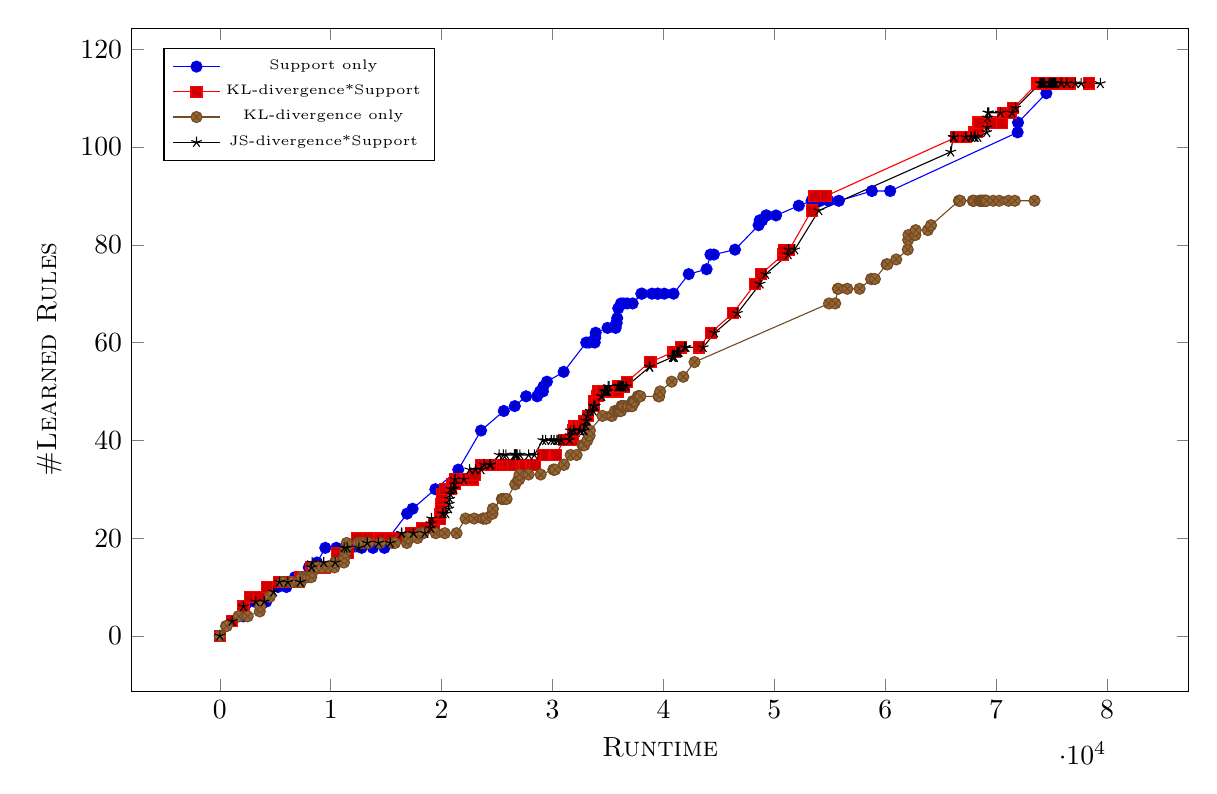
\begin{tikzpicture}
  \begin{axis}[
	width=15cm, height=10cm,
	xlabel=\textsc{Runtime},
	ylabel=\textsc{\#Learned Rules},
        legend entries={Support only, KL-divergence*Support, KL-divergence only, JS-divergence*Support},
	legend style={legend pos=north west,font=\tiny}]
      ]
  \addplot coordinates {(0,0) (1072,3) (2125,4) (3132,7) (4186,7) (5242,10) (6002,10) (6770,12) (7511,12) (8024,14)
(8763,15) (9507,18) (10503,18) (11520,18) (11785,18) (12783,18) (13803,18) (14842,18) (14886,19) (16886,25) (17380,26)
(19432,30) (21500,34) (23554,42) (25604,46) (26597,47) (27616,49) (28611,49) (28874,50) (29133,50) (29176,51) (29493,52)
(31003,54) (33035,60) (33284,60) (33802,60) (33845,61) (33889,62) (34956,63) (35695,63) (35741,64) (35782,64) (35830,65)
(35926,67) (36173,68) (36421,68) (36731,68) (37224,68) (38002,70) (38064,70) (38970,70) (39461,70) (39508,70) (40078,70)
(40913,70) (42280,74) (43891,75) (44239,78) (44545,78) (46452,79) (48579,84) (48678,85) (48899,85) (49250,86) (49295,86)
(50152,86) (52201,88) (53357,89) (53993,89) (54128,89) (54902,89) (55816,89) (58799,91) (60443,91) (71937,103)
(71971,105) (74526,111)};

  \addplot coordinates {(0,0) (1117,3) (2130,6) (2690,8) (3507,8) (4281,10) (5360,11) (6107,11) (7169,11) (7213,12)
(8212,14) (8476,14) (8503,14) (9518,14) (10552,17) (11565,17) (12334,20) (13338,20) (13381,20) (14411,20) (15450,20)
(16473,20) (17256,21) (18250,22) (19291,22) (19335,23) (19845,24) (19888,25) (19932,26) (19978,27) (20022,28) (20066,29)
(20331,30) (20861,30) (20905,31) (21166,31) (21208,32) (21483,32) (22230,32) (22257,32) (22788,32) (23042,33) (23580,35)
(23844,35) (24158,35) (24423,35) (24435,35) (24944,35) (25446,35) (25705,35) (25969,35) (26467,35) (27220,35) (27472,35)
(27515,35) (27541,35) (28048,35) (28135,35) (28398,35) (29148,37) (29413,37) (30169,37) (30195,37) (30270,37) (31034,40)
(31794,40) (31850,41) (31888,42) (31927,43) (31999,43) (32139,43) (32165,43) (32203,43) (32231,43) (32272,43) (32330,43)
(32612,43) (32699,43) (32868,44) (33162,45) (33707,47) (33733,48) (33758,48) (34013,49) (34100,49) (34138,50) (34416,50)
(34462,50) (35255,50) (35364,50) (35395,50) (35433,50) (35472,50) (35514,50) (35603,50) (35651,50) (35767,50) (35869,50)
(35909,51) (35936,51) (35963,51) (35990,51) (36030,51) (36291,51) (36319,51) (36348,51) (36429,51) (36456,51) (36717,52)
(38770,56) (38828,56) (40827,58) (40854,58) (40895,58) (40922,58) (41030,58) (41072,58) (41603,59) (43194,59) (44262,62)
(46267,66) (48275,72) (48789,74) (50807,78) (50850,79) (51350,79) (53359,87) (53598,90) (53624,90) (53662,90) (54680,90)
(66388,102) (66927,102) (67192,102) (67272,102) (68055,103) (68307,103) (68335,104) (68363,105) (68450,105) (69508,105)
(70510,105) (70551,105) (70586,107) (70681,107) (70737,107) (70802,107) (70831,107) (70872,107) (71291,107) (71555,108)
(73709,113) (73755,113) (73842,113) (73954,113) (74041,113) (74129,113) (74158,113) (74196,113) (74283,113) (74811,113)
(75329,113) (76096,113) (76622,113) (78365,113)};

  \addplot coordinates {(0,0) (558,2) (621,2) (1678,4) (1707,4) (2508,4) (3602,5) (3649,6) (4516,8) (5677,11) (6482,11)
(7023,11) (7315,11) (7389,12) (7664,12) (7947,12) (8242,12) (8343,13) (8393,14) (8710,14) (9261,14) (9793,14) (10325,14)
(10369,15) (10380,15) (11190,15) (11234,16) (11308,17) (11353,18) (11379,18) (11439,19) (12458,19) (12753,19) (13027,19)
(13383,19) (13409,19) (14448,19) (15546,19) (15793,19) (16860,19) (16925,20) (17013,20) (17820,20) (18099,21) (18354,21)
(19473,21) (20287,21) (21341,21) (22160,24) (22940,24) (23737,24) (23763,24) (23991,24) (24029,24) (24544,25) (24585,25)
(24624,26) (25425,28) (25501,28) (25607,28) (25857,28) (26640,31) (26911,32) (26961,32) (26987,32) (27026,33) (27835,33)
(28933,33) (30067,34) (30124,34) (30238,34) (31005,35) (31043,35) (31633,37) (32174,37) (32702,39) (32814,39) (32867,39)
(33142,40) (33314,41) (33341,41) (33367,42) (34498,45) (35326,45) (35352,45) (35617,46) (35865,46) (35906,46) (35980,46)
(36007,46) (36131,46) (36172,46) (36210,47) (36235,47) (36260,47) (36349,47) (36432,47) (36753,47) (36793,47) (36833,47)
(37123,47) (37149,47) (37182,47) (37225,48) (37306,48) (37386,48) (37411,48) (37683,49) (37740,49) (37767,49) (37809,49)
(37840,49) (37920,49) (39556,49) (39623,49) (39701,50) (40743,52) (41786,53) (42801,56) (54930,68) (55488,68) (55728,71)
(55766,71) (56577,71) (57688,71) (58728,73) (58754,73) (59064,73) (60120,76) (60200,76) (60993,77) (62028,79) (62066,81)
(62094,82) (62622,82) (62715,82) (62744,83) (63840,83) (64129,84) (66640,89) (66681,89) (66763,89) (67898,89) (67928,89)
(68021,89) (68488,89) (68543,89) (68584,89) (68669,89) (68757,89) (68783,89) (68907,89) (68986,89) (69017,89) (69103,89)
(69142,89) (69731,89) (70276,89) (71110,89) (71688,89) (73459,89)};

  \addplot coordinates {(0,0) (1112,3) (2136,6) (3249,7) (4009,7) (4862,9) (5375,11) (6130,11) (7246,11) (8274,14)
(8319,15) (9366,15) (10401,15) (11210,18) (11478,18) (12532,18) (13288,19) (14306,19) (15364,19) (16375,21) (16402,21)
(17457,21) (18491,21) (18999,22) (19042,23) (19085,24) (20093,25) (20134,25) (20379,25) (20643,26) (20686,27) (20730,28)
(20775,29) (20818,30) (21115,30) (21157,31) (21202,32) (22005,32) (22529,34) (23039,34) (23554,34) (23832,35) (24356,35)
(24382,35) (24420,35) (25182,37) (25566,37) (25793,37) (26560,37) (26634,37) (26663,37) (26690,37) (26778,37) (26791,37)
(27050,37) (27845,37) (28363,37) (29116,40) (29380,40) (29884,40) (30132,40) (30397,40) (30511,40) (30775,40) (31537,40)
(31575,41) (31614,42) (31878,42) (31931,42) (32443,42) (32499,42) (32537,42) (32800,42) (32831,42) (32992,43) (33020,44)
(33071,44) (33135,45) (33396,46) (33670,46) (33713,47) (33750,47) (33842,47) (34403,49) (34444,49) (34702,50) (34795,50)
(34882,50) (34908,50) (34947,50) (34974,50) (35014,51) (35094,51) (35902,51) (35991,51) (36032,51) (36070,51) (36103,51)
(36239,51) (36265,51) (36319,51) (36359,51) (36386,51) (36649,51) (38742,55) (38770,55) (40797,57) (40883,57) (40940,57)
(40984,57) (41245,58) (41276,58) (41318,58) (41377,58) (41404,58) (41916,59) (42031,59) (43579,59) (44614,62) (46672,66)
(48713,72) (49211,74) (51247,78) (51288,79) (51837,79) (54011,87) (65906,99) (66130,102) (66159,102) (66198,102)
(67254,102) (67758,102) (68021,102) (68101,102) (68351,102) (69150,103) (69180,104) (69215,106) (69244,107) (69330,107)
(70383,107) (71438,107) (71756,108) (73972,113) (74013,113) (74130,113) (74186,113) (74240,113) (74278,113) (74317,113)
(74792,113) (74819,113) (74907,113) (75017,113) (75104,113) (75186,113) (75215,113) (75254,113) (75341,113) (75869,113)
(76380,113) (77139,113) (77666,113) (79392,113)};
  \end{axis}
  \end{tikzpicture}
 % \end{minipage}
\label{fig:mdbpedia:runtime:Runtime-LearnedRules}
\end{figure}






\subsection{Example of Rules Learned}

We selected a couple of interesting rules learned with our approach in order to illustrate the kind of results we
obtain. On LinkedMDB, for example, we learned that films in English with Canadian director (first entry of
Table~\ref{tab:mdbRuleExamples}) and low budget are significantly more likely to be also Canadian than those with
higher budget. The base rule shown below has confidence $0.36$, while for the refined rule, we find the
interval $Y\leq 80000$ with confidence $0.83$, which represents a confidence gain of $2.31$.

Another interesting example, show  in the second entry of Table~\ref{tab:mdbRuleExamples} reveals that films written by
a spouse of Fritz Lang (more specifically, Thea von Harbou, who was an actress, writer, and director), and which have
long runtime are more likely to have been directed by Fritz Lang than those with shorter runtime. The base rule has
confidence $0.6$ and the refined rule with $Y\geq 6800s$ has confidence $0.82$, representing a confidence gain of
$1.37$:

\begin{table}[h!]
 \begin{center}
 \caption{Interesting rules with numerical intervals learned from DBpedia}
  \begin{tabular}{ >{\emph}r >{\raggedright}p{7cm} | c | c }
    \toprule
      & Refined Rule				& Conf 	& Gain \\
    \midrule
      country(X,canada) :-&director(X,Z), bornIn(Z,canada), language(X,english), budget(X,Y), Y$\leq 80000$ &
      0.83	& 0.36 \\ \hline
      director(X,fritzLang) :-&writer(X,Z), spouse(Z,fritzLang), runtime(X,Y), Y$\geq 6800s$ & 
      0.82	& 0.37 \\ \hline
      writer(X,sylvesterStallone) :-&starring(X,sylvesterStallone), subject(X,englishLanguageFilms),
      budget(X,Y), Y$\in [6M,31M]$ &
      0.89	& 0.48 \\ \hline
      producer(X,clintEastwood) :-&director(X,clintEastwood), starring(X,clintEastwood),
      subject(X,englishLanguageFilms), budget(X,Y), Y$\geq 13M$ &
      1.00	& 0.73 \\ \hline
      starring(X,clintEastwood) :- &budget(X,Y), director(X,clintEastwood), starring(A,clintEastwood), 
      subject(A,englishLanguageFilms), Y$\in [930K,25M]$&
      0.82	& 0.56 \\ \hline
      starring(X,Z) :-&writer(X,Z), country(X,uk), distributor(X,bbc),r untime(X,Y), Y$\leq 4080s$ &
      0.9	& 0.53 \\ \hline

    \bottomrule
  \end{tabular}
  \label{tab:mdbRuleExamples}
 \end{center}
\end{table}

Other examples of interesting rules learned from the USCensus experiment are shown in
Table~\ref{tab:uscensusRuleExamples}.

\begin{table}[h!]
 \begin{center}
 \caption{Interesting rules with numerical intervals learned from USCensus}
  \begin{tabular}{ >{\emph}r >{\raggedright}p{7cm} | c | c }
    \toprule
      & Refined Rule				& Conf 	& Gain \\
    \midrule
      sex(X,male) :-&employmentStatus(X,employed),hasEducation(X,master),hasIncome(X,Y),Y>32000 &
      0.79 & 0.52 \\ \hline
      sex(X,female) :-&employmentStatus(X,employed),hasEducation(X,master),hasIncome(X.Y),Y<3700 &
      0.79 & 0.48\\ \hline
      [more to be added] & & & \\
    \bottomrule
  \end{tabular}
  \label{tab:uscensusRuleExamples}
 \end{center}
\end{table}


\subsection{Conclusion}

The results obtained in the first experiment indicate the proposed divergence combined with support measures have the
potential to be used as heuristics in order to reduce the search space of rules with numerical and categorical
constants, being much more efficient than support only or divergence only.

In our last experiment, we apply it into the core-ILP and try to evaluate our proposed ILP extension on LinkedMDB and
DBpedia. Results indicate that indeed, with the divergence measures, the precision of the interestingness predictions
is higher for lower recall. Moreover, KL-divergence*support seems to perform slightly better than JS-divergence*support.
However, since the data is not ideal, it is premature to draw any conclusions. 
[Elaborate later]

[Separete section?]

- UScensus experiment shows the advantage of combining divergence with support

- DBpedia LinkedMDB not very conclusive

- 

\subsection{Future Work}

[???]

- Experiments with better data?

- Extend the proposed technique to multidimensions































\begin{comment}
\begin{figure}
 \caption{Precision - Recall }
 \centering
 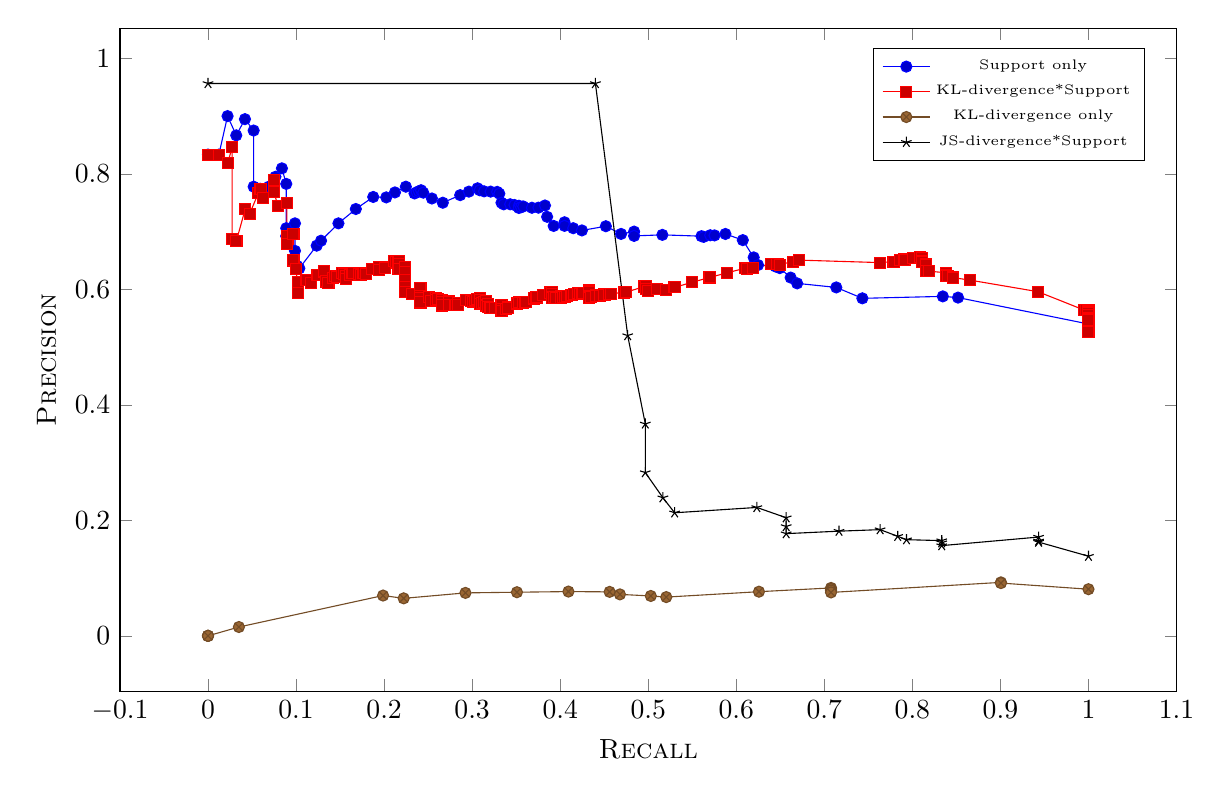
\begin{tikzpicture}[scale=1.0]
  \begin{axis}[
	width=15cm, height=10cm,
	xlabel=\textsc{Recall},
	ylabel=\textsc{Precision},
	legend entries={Support only, KL-divergence*Support, KL-divergence only, JS-divergence*Support},
	legend style={legend pos=north east,font=\tiny}]
      ]
%  \addplot coordinates {(0,0.08527132) (0.03741496,0.08527132) (0.4591837,0.5212355) (0.4795918,0.3691100)
%(0.4931973,0.3072034)
%(0.5136054,0.2581197) (0.547619,0.2303290) (0.6360544,0.2379135) (0.6360544,0.2080089) (0.6768708,0.2090336)
%(0.6972789,0.193032) (0.7517007,0.1957484) (0.7653061,0.1810137) (0.7653061,0.1781473) (0.7959183,0.1696882)
%(0.8027211,0.1621993) (0.8027211,0.1587088) (0.9013606,0.1726384) (0.9421769,0.1716233) (0.9421769,0.1653731)
%(1.0,0.1418234)};

    \addplot coordinates {(0,0.8333333) (0.01234568,0.8333333) (0.02222222,0.9) (0.03209877,0.8666667)
(0.04197531,0.8947368) (0.05185185,0.875) (0.05185185,0.7777778) (0.05679012,0.7666667) (0.05925926,0.7741935)
(0.06419753,0.7647059) (0.0691358,0.7777778) (0.07654321,0.7948718) (0.08395062,0.8095238) (0.08888889,0.7826087)
(0.08888889,0.7058824) (0.08888889,0.6923077) (0.09876543,0.7142857) (0.09876543,0.6666667) (0.1012346,0.640625)
(0.1037037,0.6363636) (0.1234568,0.6756757) (0.1283951,0.6842105) (0.1481482,0.7142857) (0.1679012,0.7391304)
(0.1876543,0.76) (0.2024691,0.7592593) (0.2123457,0.7678571) (0.2246914,0.7777778) (0.2345679,0.766129)
(0.2370370,0.768) (0.2395062,0.7698413) (0.2419753,0.7716535) (0.2444444,0.7674419) (0.254321,0.757353) (0.2666667,0.75)
(0.2864197,0.7631579) (0.2962963,0.7692308) (0.3061728,0.775) (0.308642,0.771605) (0.3135802,0.769697)
(0.3209876,0.7692308) (0.3283951,0.7687861) (0.3308642,0.7657143) (0.3333333,0.75) (0.3358025,0.7472528)
(0.3432099,0.7473118) (0.3481481,0.7460318) (0.3530864,0.7447917) (0.3530864,0.7409326) (0.3555556,0.742268)
(0.3580247,0.7435898) (0.3679012,0.7412935) (0.3753086,0.7414634) (0.3827161,0.7451923) (0.3851852,0.7255814)
(0.3925926,0.7098214) (0.4049383,0.7161572) (0.4049383,0.7099567) (0.4148148,0.7058824) (0.4246914,0.7020408)
(0.4518518,0.7093023) (0.4691358,0.6959707) (0.4839506,0.7) (0.4839506,0.6925795) (0.5160494,0.6943521)
(0.5604938,0.6920732) (0.562963,0.6909091) (0.5703704,0.6936937) (0.5753086,0.6934524) (0.5876543,0.6959065)
(0.6074074,0.6852367) (0.619753,0.6553525) (0.6246914,0.642132) (0.6444445,0.6397059) (0.6493827,0.6368039)
(0.6617284,0.6203704) (0.6691358,0.6103604) (0.7135803,0.6033403) (0.7432099,0.584466) (0.8345679,0.5878261)
(0.8518519,0.5857385) (1,0.54)};

%   \addplot coordinates { (0,0.9538462) (0.4290657,0.9538462) (0.467128,0.5212355) (0.4878893,0.3691100)
%(0.4878893,0.2848485) (0.4878893,0.2508897) (0.4878893,0.2227488) (0.5086505,0.1970509) (0.5224913,0.180622)
%(0.6124567,0.1917660) (0.6470588,0.1803279) (0.6885813,0.1825688) (0.7439446,0.1858254) (0.7647059,0.1744278)
%(0.799308,0.1676343) (0.8408305,0.1667810) (0.8408305,0.1631968) (0.8408305,0.1583062) (0.9411765,0.1718256)
%(0.9411765,0.1654501) (0.9411765,0.1634615) (1.0,0.1401552)};

   \addplot coordinates {(0,0.8333333) (0.01243781,0.8333333) (0.02238806,0.8181818) (0.02736319,0.8461539)
(0.02736319,0.6875) (0.03233831,0.6842105) (0.04228856,0.7391304) (0.04726368,0.7307692) (0.05721393,0.7666667)
(0.05970149,0.7741935) (0.06218905,0.7575757) (0.07462686,0.7894737) (0.07462686,0.7692308) (0.07960199,0.744186)
(0.08955224,0.75) (0.08955224,0.6923077) (0.08955224,0.6792453) (0.09701493,0.6964286) (0.09701493,0.65)
(0.09950249,0.6349207) (0.1019900,0.6119403) (0.1019900,0.5942029) (0.1119403,0.6164383) (0.1169154,0.6103896)
(0.1243781,0.625) (0.1318408,0.6309524) (0.1343284,0.6136364) (0.1368159,0.6111111) (0.1417911,0.6195652)
(0.1442786,0.6236559) (0.1467662,0.6210526) (0.1517413,0.628866) (0.1542289,0.6262626) (0.1567164,0.6237624)
(0.1567164,0.617647) (0.1616915,0.625) (0.1641791,0.6285715) (0.1716418,0.6272727) (0.1741293,0.625)
(0.1766169,0.6283186) (0.1791045,0.626087) (0.1865672,0.6355932) (0.1940299,0.6393443) (0.1940299,0.6341463)
(0.2014925,0.6377953) (0.2114428,0.648855) (0.2139303,0.6466165) (0.2164179,0.6492537) (0.2164179,0.6444445)
(0.2164179,0.6350365) (0.2238806,0.6382979) (0.2238806,0.6293706) (0.2238806,0.6164383) (0.2238806,0.6040269)
(0.2238806,0.5960265) (0.2313433,0.5923567) (0.2412935,0.6024845) (0.2412935,0.5878788) (0.2412935,0.5843373)
(0.2412935,0.577381) (0.2512438,0.5872093) (0.2537313,0.5795454) (0.2587065,0.5842696) (0.2587065,0.5810056)
(0.261194,0.5833333) (0.2661692,0.5815217) (0.2661692,0.5783784) (0.2661692,0.5721925) (0.2736318,0.5789474)
(0.2736318,0.5729167) (0.2810945,0.573604) (0.2835821,0.5757576) (0.2835821,0.5728643) (0.2935323,0.5812808)
(0.2985075,0.5797101) (0.300995,0.5817308) (0.300995,0.5789474) (0.3034826,0.5809524) (0.3059702,0.5829384)
(0.3084577,0.5849057) (0.3084577,0.5821596) (0.3084577,0.5740741) (0.3109453,0.5760369) (0.3134328,0.5779817)
(0.3159204,0.5799087) (0.3159204,0.5720721) (0.3184079,0.5739911) (0.3184079,0.5688889) (0.3208955,0.568282)
(0.3258706,0.5670996) (0.3333333,0.5726496) (0.3333333,0.5654008) (0.3333333,0.5630252) (0.3383084,0.5666667)
(0.340796,0.5684648) (0.3507463,0.5755102) (0.3532338,0.5772358) (0.3582090,0.5783132) (0.3582090,0.576)
(0.3606965,0.5776892) (0.3706468,0.5843137) (0.3731343,0.5859375) (0.380597,0.5907336) (0.3880597,0.5954198)
(0.3880597,0.5931559) (0.3905473,0.594697) (0.3905473,0.5924528) (0.3905473,0.5858209) (0.3930348,0.5873606)
(0.3955224,0.5845588) (0.4004975,0.5875912) (0.4004975,0.5854545) (0.4029851,0.5869565) (0.4054726,0.586331)
(0.4079602,0.5878136) (0.4129353,0.5907474) (0.4154229,0.5921986) (0.420398,0.5929825) (0.4228856,0.5923345)
(0.4253731,0.59375) (0.4328358,0.5979381) (0.4328358,0.5958904) (0.4328358,0.5878378) (0.4328358,0.5858586)
(0.4353234,0.5872483) (0.4402985,0.59) (0.4402985,0.5880399) (0.4452736,0.5907591) (0.4452736,0.5888158)
(0.4502487,0.5915033) (0.4502487,0.5895765) (0.4552239,0.592233) (0.4577114,0.5916399) (0.4726368,0.5956113)
(0.4726368,0.59375) (0.4751244,0.5950156) (0.4950249,0.6048632) (0.4975124,0.6060606) (0.4975124,0.6006006)
(0.5,0.5964392) (0.5099502,0.601173) (0.5199005,0.5988539) (0.5298507,0.6033995) (0.5497512,0.6121883)
(0.5696517,0.6205962) (0.5895522,0.6286472) (0.6094527,0.6363636) (0.6119403,0.6356589) (0.619403,0.6368287)
(0.6393035,0.6441103) (0.6467662,0.6435643) (0.6492537,0.6428571) (0.6641791,0.6480582) (0.6716418,0.6506024)
(0.7636816,0.6463158) (0.778607,0.6480331) (0.7860696,0.6502058) (0.7910448,0.6516393) (0.800995,0.6544715)
(0.8084577,0.6552419) (0.8109453,0.6546185) (0.8109453,0.6481113) (0.8159204,0.6444008) (0.8159204,0.6418787)
(0.8159204,0.6319846) (0.818408,0.631478) (0.8383084,0.6287314) (0.8383084,0.6240741) (0.8383084,0.6229205)
(0.840796,0.6236162) (0.840796,0.6224678) (0.8457711,0.620438) (0.8656716,0.6159292) (0.9427861,0.5959119)
(0.9950249,0.5641749) (0.9975125,0.5639943) (1,0.5638149) (1,0.5622377) (1,0.5614525) (1,0.5583333) (1,0.5552486)
(1,0.5506849) (1,0.5476839) (1,0.526178)};

  \addplot coordinates {(0,0) (0,0) (0,0) (0,0) (0.03508772,0.01530612) (0.1988304,0.0698152) 
  (0.2222222,0.06495727) (0.2923977,0.07440476) (0.3508772,0.07556675) (0.4093567,0.07667032) (0.4561403,0.07617188)
(0.4678363,0.07181329) (0.502924,0.06907631) (0.5204678,0.06711916) (0.625731,0.0764832) (0.7076023,0.0829904)
(0.7076023,0.0810992) (0.7076023,0.07846952) (0.7076023,0.07520199) (0.9005848,0.09260373)
 (0.9005848,0.09139466) (1.0,0.08077468)};

 \addplot coordinates {(0,0.9565217) (0.44,0.9565217) (0.4766667,0.52) (0.4966667,0.3669951) 
(0.4966667,0.2827325) (0.5166667,0.2391975) (0.53,0.2131367) (0.6233333,0.2223543) (0.6566667,0.2045691)
 (0.6566667,0.1894231) (0.6566667,0.1769991) (0.7166666,0.1812816) (0.7633333,0.1839358) (0.7833334,0.1724138)
 (0.7933334,0.1665500) (0.8333333,0.1649076) (0.8333333,0.1612903) (0.8333333,0.15625) (0.9433333,0.1711004) 
 (0.9433333,0.1644393) (0.9433333,0.1623637) (1.0,0.1379310)};


  \end{axis}
  \end{tikzpicture}
\label{fig:mdbpedia:Precision-Recall}
\end{figure}

\begin{figure}
 \caption{Runtime-LearnedRules}
 \centering
 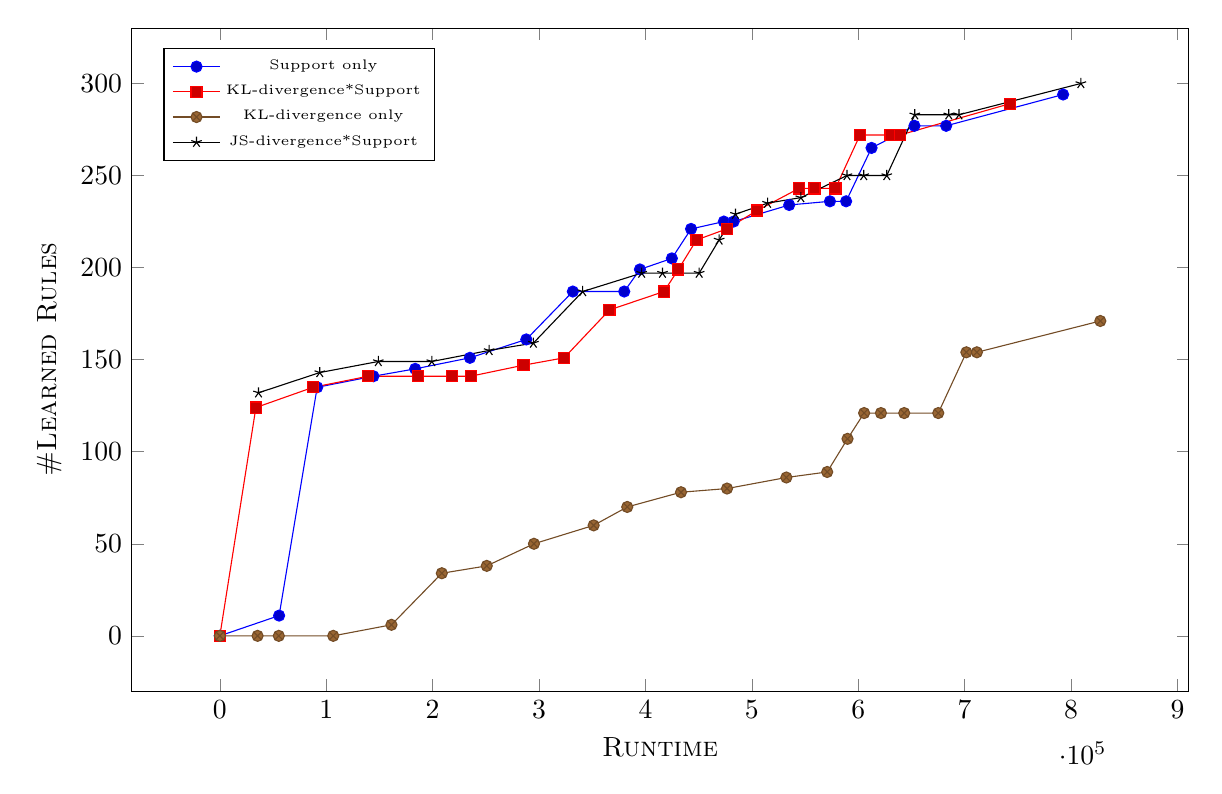
\begin{tikzpicture}[scale=1.0]
  \begin{axis}[
	width=15cm, height=10cm,
	xlabel=\textsc{Runtime},
	ylabel=\textsc{\#Learned Rules},
        legend entries={Support only, KL-divergence*Support, KL-divergence only, JS-divergence*Support},
	legend style={legend pos=north west,font=\tiny}]
      ]
  \addplot coordinates {(0.0,0.0) (55709,11) (91488,135) (144319,141) (183567,145) (235053,151) (288040,161)
(331747,187)
(380080,187) (394814,199)
(424827,205) (442860,221) (473691,225) (482918,225) (535099,234) (573386,236) (588600,236) (612505,265) (652833,277)
(682636,277) (792557,294)};

  \addplot coordinates {(0.0,0.0) (33892,124) (87747,135) (139353,141) (186294,141) (217893,141) (235750,141)
(285443,147)
(323626,151) (366197,177) (417438,187) (430932,199) (447970,215) (476371,221) (504948,231) (544307,243) (558897,243)
(578569,243) (601647,272) (630384,272) (639120,272) (742514,289)};
 
  \addplot coordinates {(0.0,0.0) (35466,0.0) (55421,0.0) (106586,0.0) (161302,6) (208629,34) (250863,38) (295212,50)
(351300,60)
(382899,70) (433423,78) (476677,80) (532442,86) (570818,89) (589925,107) (605518,121) (621333,121) (643190,121)
(675208,121) (701631,154) (711515,154) (827520,171)};

 \addplot coordinates { (36343,132) (93944,143) (148944,149) (199223,149) (253104,155) (294678,159) (341024,187)
(396459,197) (416000,197) (450504,197) (469231,215) (484591,229) (514785,235) (546069,238) (589417,250) (605128,250)
(626821,250) (653140,283) (685085,283) (694687,283) (809238,300)};

  \end{axis}
  \end{tikzpicture}
\label{fig:mdbpedia:Runtime-LearnedRules}
\end{figure}







 \begin{figure}
\caption{Lattices with 3 levels}
\centering
\begin{tikzpicture}[scale=1.0]
 \begin{axis}[
	width=15cm, height=10cm,
        xlabel=\textsc{\#Nodes per lattice level},
        ylabel=\textsc{Time to build lattice ($ms$)}
    ]
\addplot coordinates {(5,2165) (10,4337) (15,6723) (20,8860) (30,11969) (40,14626) (50,21288) (60,22329) (70,24577)
(80,25387) (90,27539) (100,30210)};
\addplot coordinates {(5, 235) (10,748) (15, 1317) (20, 1590) (30, 1890) (40, 2482) (50, 3182) (60, 3474) (70, 4020)
(80, 4911) (90,5982) (100,6684)};
\end{axis}
\end{tikzpicture}
\end{figure}

\begin{figure}
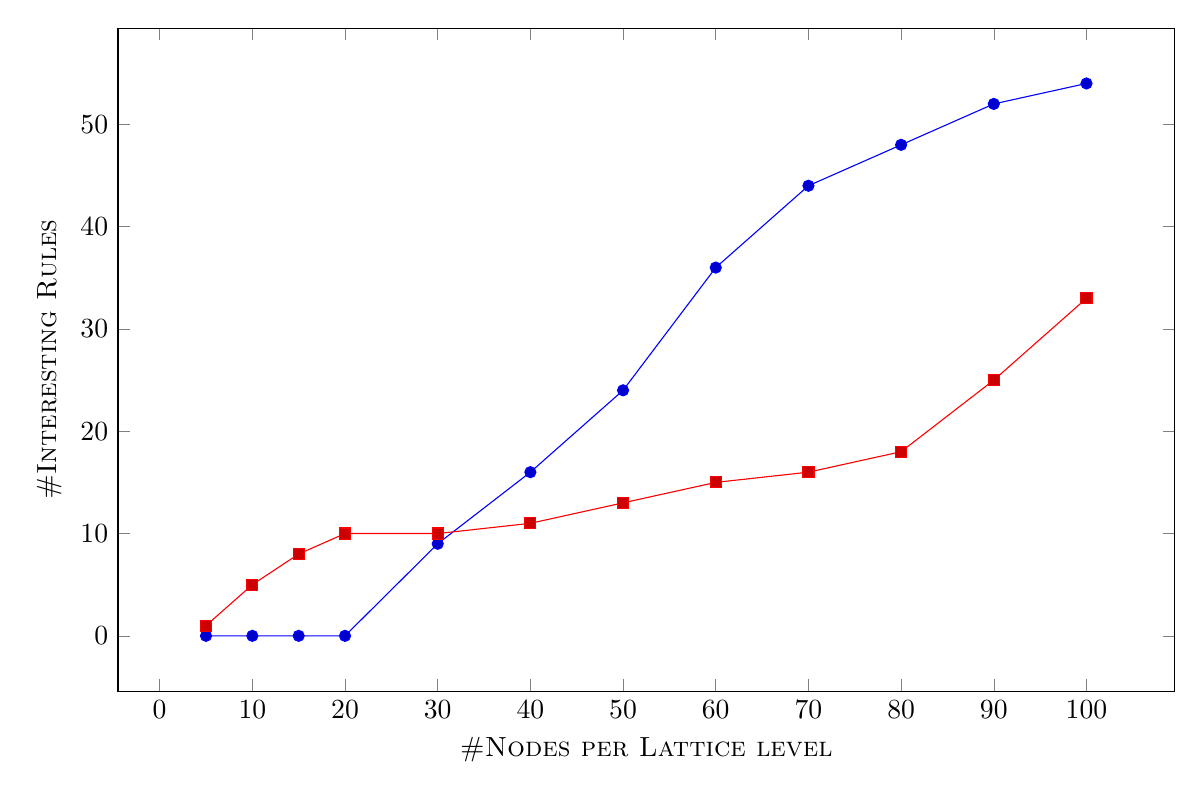
\begin{tikzpicture}[scale=1.0]
 \begin{axis}[
	width=15cm, height=10cm,
        xlabel=\textsc{\#Nodes per Lattice level},
        ylabel=\textsc{\#Interesting Rules}
    ]
\addplot coordinates {(5,0.0) (10,0.0) (15,0.0) (20, 0) (30, 9) (40,16) (50,24) (60,36) (70,44) (80,48) (90,52)
(100,54)};
\addplot coordinates {(5,1.0) (10,5) (15,8) (20,10) (30,10) (40,11) (50,13) (60,15) (70,16) (80,18) (90,25) (100,33)};
\end{axis}
\end{tikzpicture}
\end{figure}


\begin{figure}
 \caption{Lattice with 4 levels}
 \centering
 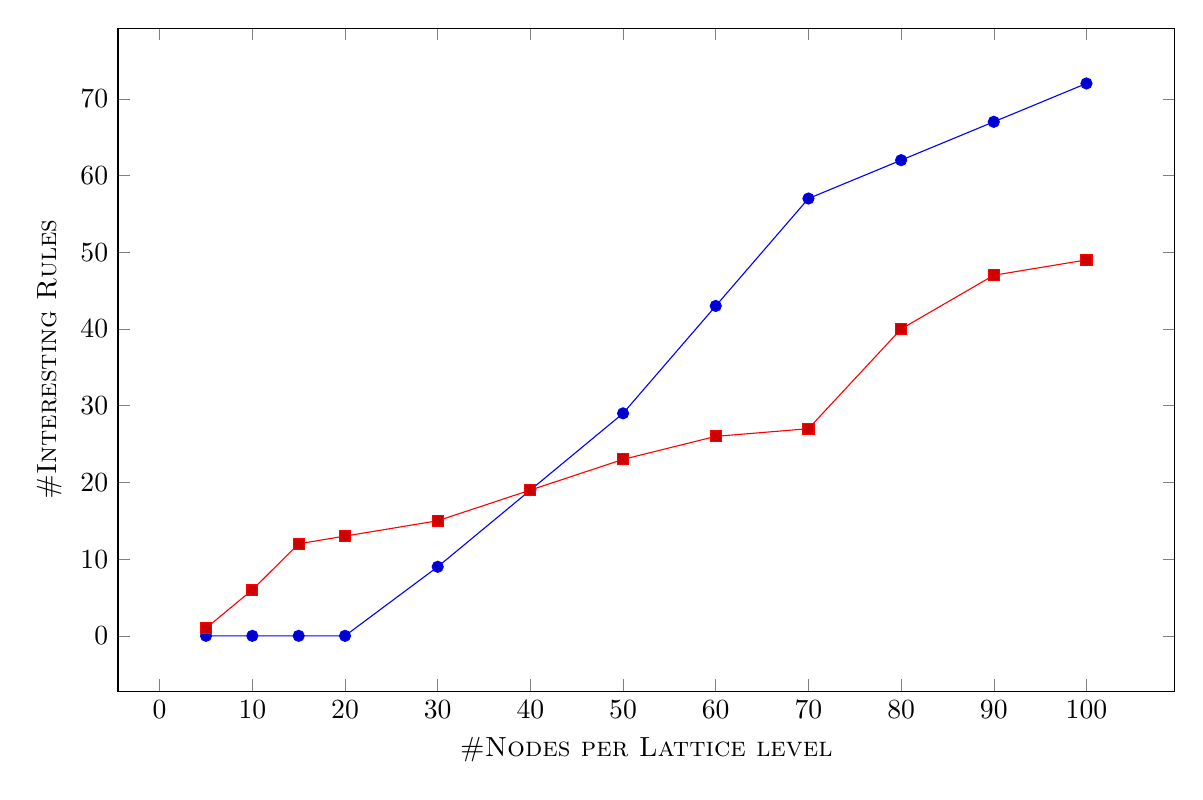
\begin{tikzpicture}[scale=1.0]
  \begin{axis}[
	  width=15cm, height=10cm,
	  xlabel=\textsc{\#Nodes per Lattice level},
	  ylabel=\textsc{\#Interesting Rules}
      ]
  \addplot coordinates {(5,0.0) (10,0.0) (15, 0) (20, 0) (30, 9) (40,19) (50,29) (60,43) (70,57) (80,62) (90,67)
(100,72)};
  %(110,75) (120,79) (130,84) (140,88) (150,94) (200,122) (250,159) (300,178) (350,200) (400,214) (450,231) (500,242)};
  \addplot coordinates {(5,1.0) (10,6) (15,12) (20,13) (30,15) (40,19) (50,23) (60,26) (70,27) (80,40) (90,47)
(100,49)};
  %(110,) (120,) (130,) (140,) (150,) (200,) (250,) (300,) (350,) (400,) (450,) (500,)};
  \end{axis}
  \end{tikzpicture}
\end{figure}

\begin{figure}
  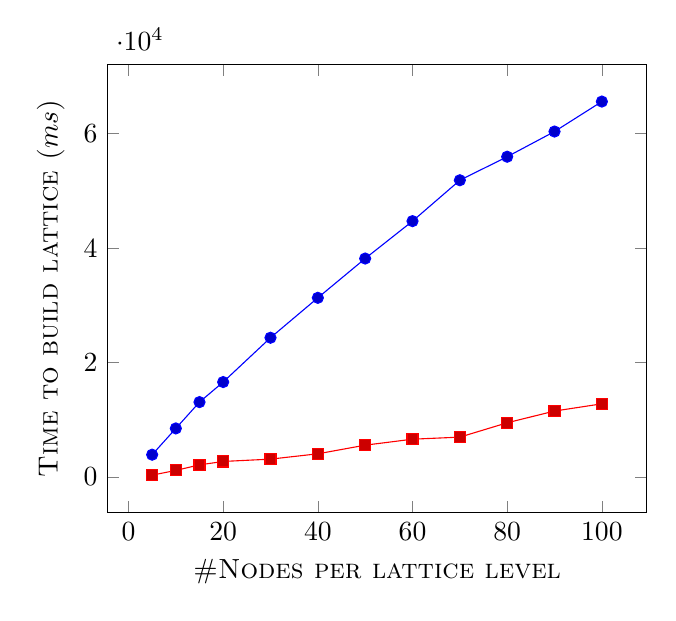
\begin{tikzpicture}[scale=1.0]
  \begin{axis}[
	  xlabel=\textsc{\#Nodes per lattice level},
	  ylabel=\textsc{Time to build lattice ($ms$)}
      ]
  \addplot coordinates {(5,3905) (10,8496) (15,13097) (20,16601) (30,24348) (40,31322) (50,38189) (60,44724) (70,51869)
  (80,55981) (90,60382) (100,65622)};
% (110,75) (120,79) (130,84) (140,88) (150,94) (200,122) (250,159) (300,178)  (350,200) (400,214) (450,231) (500,242)};
  \addplot coordinates {(5, 330) (10,1161) (15, 2128) (20, 2722) (30, 3130) (40, 4060) (50, 5571) (60, 6613) (70, 6976)
  (80, 9483) (90,11534) (100,12795)};
% (110,) (120,) (130,) (140,) (150,) (200,) (250,) (300,) (350,) (400,) (450,) (500,)};
  \end{axis}
  \end{tikzpicture}
\end{figure}
\end{comment}



